\chapter{Monte Carlo Simulation}
The primary references used for writing this chapter were \cite{MC_ref1,MC_ref2,MC_ref3,schnoor_thesis,Seymour}. These should be consulted for further reading.

Monte Carlo simulations are logically divided into two classes: event generation and detector simulation. Event generators attempt to simulate the particle interactions and their kinematics with the resulting output being fed as input into detector simulators. Some of the most commonly used GPMC (General-Purpose Monte Carlo) event generators are \textsc{Herwig} \cite{Herwig}, \textsc{PowHeg-Box} \cite{Powheg}, \textsc{Pythia} \cite{Pythia}, \textsc{Sherpa} \cite{Sherpa}, and \textsc{Madgraph} \cite{Madgraph}. The detector simulators then subsequently model how the event generator output will interact with the detector. \textsc{GEANT4} \cite {GEANT} is an example of a detector simulator package.
\section{Event Generators}
\label{event_generators}
Monte Carlo (MC) event generators are a powerful and commonly used tool in high energy physics that randomly generate events by sampling them from some \emph{a priori} parent distribution. They attempt to simulate high energy collisions in collider experiments and thus provide essential predictions of such physics processes which are useful to both experimentalists and theorists alike. Experimentalists in particular, rely on the predictions gained from event generators in order to search for new physics. Event generators are often used in conjunction with detector simulators in order to predict how the detector will respond in the event of a real high energy collision. 

The very brief overview of MC event generators given here is concerned specifically with generators which simulate hard proton-proton (p-p) collisions at high (in excess of several hundred GeV) centre of mass energies. Such collisions result in a large number of particles in the final state which can trace their evolution back to the original p-p collision. MC event generators are able to simulate the final states, providing descriptions of the types of particle present as well as the kinematics of those particle on an event-by-event basis \cite{MC2}.

Event generators typically take into account:
\begin{itemize}
\item the matrix-element of the \emph{hard process} (the process with the highest momentum scale),
\item the inclusion of higher-order QCD and QED (Quantum Electrodynamics) effects via \emph{parton shower} algorithms,
\item \emph{hadronisation}, which must be described by non-perturbative QCD,
\item effects from the \emph{underlying event}.
\end{itemize}

In simulating data events taken by the ATLAS detector, the events are classified into three successive levels. Events on the truth level include information on objects derived solely from the hard process perturbative QCD theory, i.e. excluding the parton shower or hadronisation stages of event simulation (see section \ref{event_generators}). The subsequent level, the Final state level events include information on stable objects after the hadronisation step, be they originating from the hard process directly, or indirectly via the parton shower or hadronisation algorithms. Objects associated with the underlying event are included here too. The final Reconstruction level has information on objects reconstructed by algorithms run on complete detector simulated events, including material effects and magnetic fields. This is represented visually in figure \ref{mc_levels}.
\begin{figure}
\centering
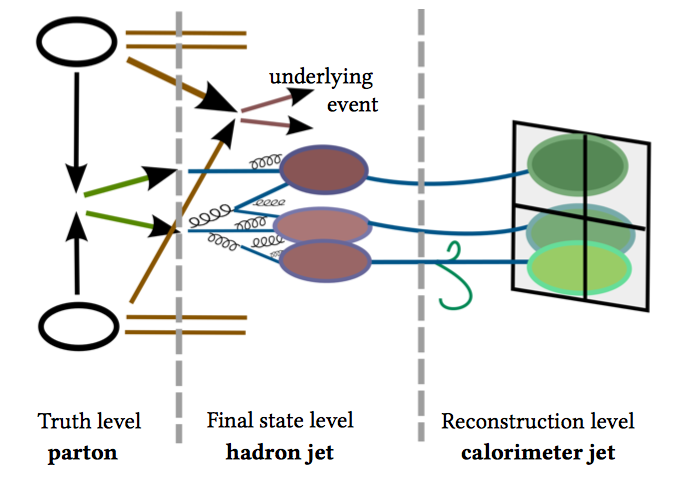
\includegraphics[scale=0.5]{images/sim_levels}
\caption{Illustration of the levels used in describing MC simulated high-energy collisions in the ATLAS detector. \cite{schnoor_thesis}}
\label{mc_levels}
\end{figure}
\subsection{The Hard Process}
In QED, calculations involve summing contributions from increasingly higher-order Feynman diagrams (i.e. perturbation theory), with the sum converging due to exponential dependence on the QED coupling constant $\alpha_{e}$  and the fact that $\alpha_{e} < 1$. This is not, in general, the case in QCD, where the running coupling constant $\alpha_{s}$ can exceed unity. This physically represents the confinement of quarks and gluons within hadrons. However, in special cases where, at sufficiently high energies and small distances, $\alpha_{s}$ decreases with the renormalisation scale $\mu_{R}$ until $\alpha_{s}$ becomes less than unity in what is called asymptotic freedom. The partons (quarks and gluons) can now be treated as free particles and perturbative QCD is applicable.

The \emph{factorisation therem} \cite{SM3} can be used in order to separate the sub-processes in a high energy scatter, into an infrared safe part (i.e. not dependent on the unknown, long-distance properties of QCD where perturbation theory breaks down) and a non-infrared safe part. For a scattering process $ab \longrightarrow n$, with initial hadronic particles $a$, $b$, and final state particles $n$, (illustrated in figure \ref{factorisation_theorem}), the factorisation theorem yields:
\begin{equation}
\sigma_{ab \rightarrow n} = \sum_{a,b}\int^{1}_{0}dx_{x}dx_{b}\int \underbrace{f_{a}^{h_{1}}(x_{a},\mu_{F})f_{b}^{h_{2}}(x_{b},\mu_{F})}_{\text{non-perturbative}}\underbrace{d\hat{\sigma}_{ab \rightarrow n}(\mu_{F},\mu_{R})}_{\text{perturbative}}.
\end{equation}
While the perturbation part can be calculated by treating the partons as free particles, the non-perturbative part must be inferred from the parton distribution functions (PDFs) $f_{i}^{h}(x_{i},\mu_{F})$ of the initial parton with respect to the original hadron $h$ with Bjorken $x_{i}$ and factorisation scale $\mu_{F}$. The PDF is the probability of finding a parton $i$, with Bjorken $x_{i}$ in a hadron $h$, at a energy scale $\mu_{F}$. The perturbative part constitutes the matrix element $| \mathcal{M}_{ab\rightarrow n} |^{2}$, so the cross-section be factorised as an integral over the final-state phase space $\Phi_{n}$:
\begin{equation}
\sigma_{ab \rightarrow n} = \sum_{a,b}\int^{1}_{0}dx_{x}dx_{b}\int d\Phi_{n} f_{a}^{h_{1}}(x_{a},\mu_{F})f_{b}^{h_{2}}(x_{b},\mu_{F}) \times \frac{1}{2\hat{s}}| \mathcal{M}_{ab\rightarrow n} |^{2} (\Phi _{n} ; \mu_{F},\mu_{R}).
\end{equation}
So the factorisation method allows for the cross-section to be calculated at the cost  of introducing a dependence on $\mu_{F}$. This is a very high dimensional integral and methods of MC integration are used for practicality.
\begin{figure}
\centering
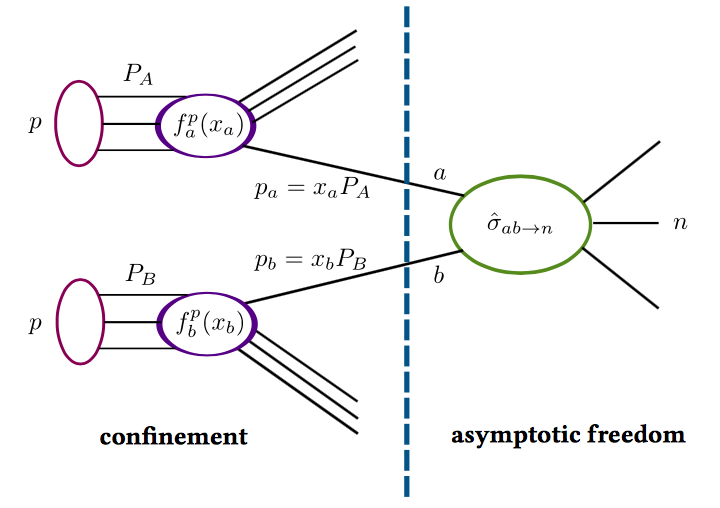
\includegraphics[scale=0.5]{images/factorisation_theorem.png}
\caption{An illustration of the factorisation theorem, showing how to the cross-section of a hadronic collision can be separated into a short distance part (where perturbative QCD is applicable) and a long distance part (where non-perturbative QCD must be used). \cite{schnoor_thesis}}
\label{factorisation_theorem}
\end{figure}
\subsection{Higher-Order Effects}
The final state particles from the evaluation of the fixed-order matrix-element are stable leptons and (non-observable) partons. Higher-order effects must be included to describe hadronisation, unstable particle decays, and the underlying event. These are each shown as components of a \textsc{Sherpa} simulated event in figure \ref{sherpa_event_sim}.
\begin{figure}
\centering
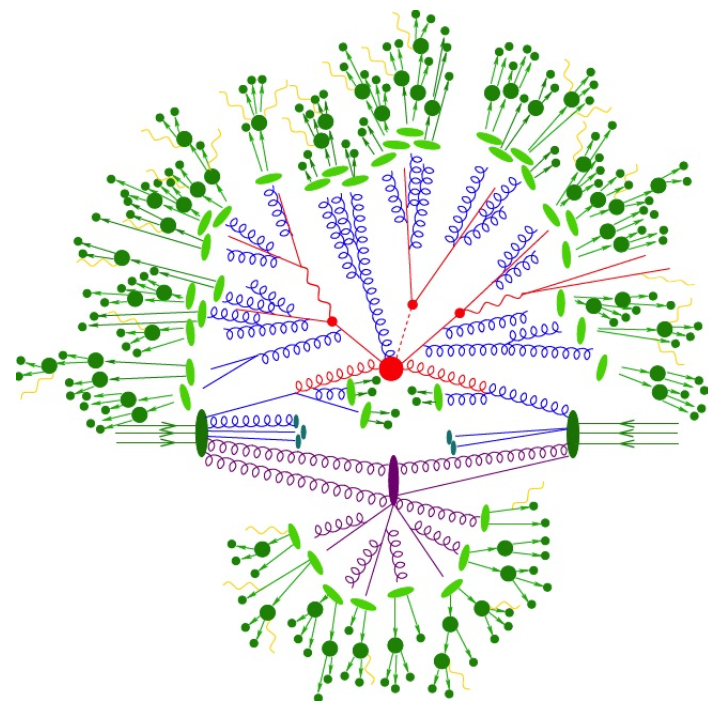
\includegraphics[scale=0.4]{images/sherpa_event_sim.png}
\caption{An illustration of a \textsc{Sherpa} generated event simulation. The hard interaction is shown in red, the partonic shower products in blue, the hadronised partons in green, hadronic decays in dark green, and the QED radiation in yellow. Note also the presence of the underlying event, coloured purple. \cite{SHERPA_image}}
\label{sherpa_event_sim}
\end{figure}
\subsubsection{Parton Shower}
Higher-order QCD effects can come from a parton showering and hadronisation algorithm. Parton showering is a complex process to simulate, as gluons carry colour and thus can trigger new additional QCD processes. Starting from the hard process (the process with the highest momentum scale), the parton shower simulation proceeds to successively lower momentum scales until the threshold of where perturbation theory is longer applicable is reached.
\subsubsection{Hadronisation}
The partons that result from the parton showering algorithm proceed to form colour-less bound states (hadrons), as described by the hadronisation algorithm. Unfortunately, hadronisation falls outside the region where perturbative QCD is applicable. As a result, hadronisation relies on QCD-inspired phenomenological models. Examples of such models are the \emph{string model} \cite{string_model}, which is based on linear confinement of partons, and the \emph{cluster model} \cite{cluster_model}, which is based on the pre-confinement of parton showers.
\subsubsection{Hadron and $\uptau$-Lepton Decays}
Many of the resulting hadrons that form, as described by the hadronisation algorithms, are unstable. These will decay before they can be directly measured by the detector. As a result, algorithms closely related to those used to model hadronisation, are used to simulate these hadronic decays. $\uptau$-leptons, produced in the original hard scattering process, also decay before they can be directly measured \cite{ATLAS}. Decay algorithms, that take into account spin effects, are used to simulate $\uptau$-lepton decays.
\subsubsection{QED Radiation}
QED radiation contributions are modeled in a similar way as the QCD parton shower but with electric charge in place of colour charge. Alternatively, the \emph{YFS formalism} \cite{YFS}, which is based on multipole evolution, can be used.
\subsubsection{Underlying Event}
Here the effects from the highly probable secondary interactions between proton remnants are considered. In the laboratory frame, the two colliding protons flatten into thin discs due to Lorentz contraction. The collision occurs when these two discs are approximately overlapping each other in space-time. This results in it being very likely that there will be other interactions aside from the hard process. These other processes are referred to as the underlying event. The hadrons that result contaminate the hard process. The underlying event is generally modeled in terms of additional interactions between the partons of the colliding protons.
\section{GEANT4: A Detector Simulator}
Simulating a detector's response to simulated data helps understand and optimise the way it will respond to actual physical processes and scenarios. The particles which result from a hard scatter will interact with the detector through random processes such as pair production, hadronic interactions with detector material, Coloumb scattering, or ionisation. Programming packages like GEANT4 (GEometry ANd Tracking) use MC techniques to simulate the passage of hard scatter products though detectors and gauge their response. To effectively simulate a detector, programming packages require descriptions of the detector's geometry and constituent material.

GEANT4 is a freely available toolkit used for simulating the passage of particles through matter. GEANT4 also provides a graphical representation of the experimental setup as well as the particles' trajectories. The experimental setup is described by the user in terms of geometrical volumes. The constituent materials of these volumes are also user-specified as this is required for GEANT4 to accurately model the detector's response to the traversing particles.

A basic summary of the working of GEANT4 is given here. Please see the documentation \cite{GEANT} for details. GEANT4 detector simulation is logically divided into three phases:
\begin{enumerate}
\item \textit{Initialisation}
\item \textit{Event Processing}
\item \textit{Termination}
\end{enumerate}
In \textit{Initialisation} GEANT4 prepares for particle transport. All geometrical information provided by the user is processed. Tables for energy loss and cross-section are computed and stored. Properties of the relevant particles and characteristics of the detector materials are also stored. In \textit{Event Processing}, each event is initialised, processed, and then cleaned from memory. Each particle is propagated through the setup and the detector's responses are simulated. These responses are stored along with the kinematics of the event. Once all events have been processed, GEANT4 proceeds to the final phase. The \textit{Termination} phase is user-controlled and commonly just computes and prints some statistical and technical information related to the preceding run.
\begin{figure}
\centering
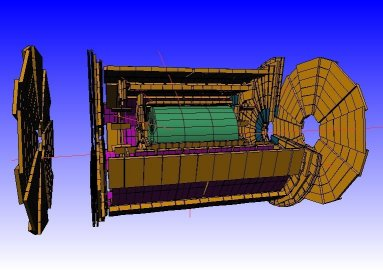
\includegraphics[scale=0.5]{images/geant_atlas.jpg}
\caption{GEANT4-created visualisation of the ATLAS detector. \cite{geant_atlas}}
\label{event_generator}
\end{figure}
\section{Simulation of the ATLAS Detector}
The actual application of the ATLAS detector simulation is done via the simulation chain, shown in figure \ref{sim_chain}. Initially, an MC generator generates events in \emph{HepMC} \cite{HEPMC} format. Next, events pass through the particle filter which applies some kinematic requirements. In the MCTruth (Gen) stage, the detector simulation uses generator level information, called MC truth, in order to simulate energy deposit signals. These simulated energy deposit are stored, along with their spatial coordinates, in ``Hits'' files. This forms part of the MC truth record. Similarly, in the simulation stage\footnote{This is the most computationally expensive step, taking several minutes per event.}, information of tracks and particle decays are also stored in the MC truth record. Simulated Data Objects (SDOs) are used to store associations between generator-level particles and simulated detector hits. Subsequently, the simulated analogue signals stored in the ``Hits'' files are converted into simulated digital signals that mimic those outputted from the detector Read-Out Drivers (RODs). At the same time, simulated pile-up contributions are added to the MC truth record. In the ultimate reconstruction step, the events are stored in bytestream format, to be subsequently converted into the Raw Data Objects (RDOs). It is important that they have the same format as actual data events recorded by the ATLAS detector, in order for the simulated data to be useful for calibration purposes and predicting the behaviour of real data.
\begin{figure}
\centering
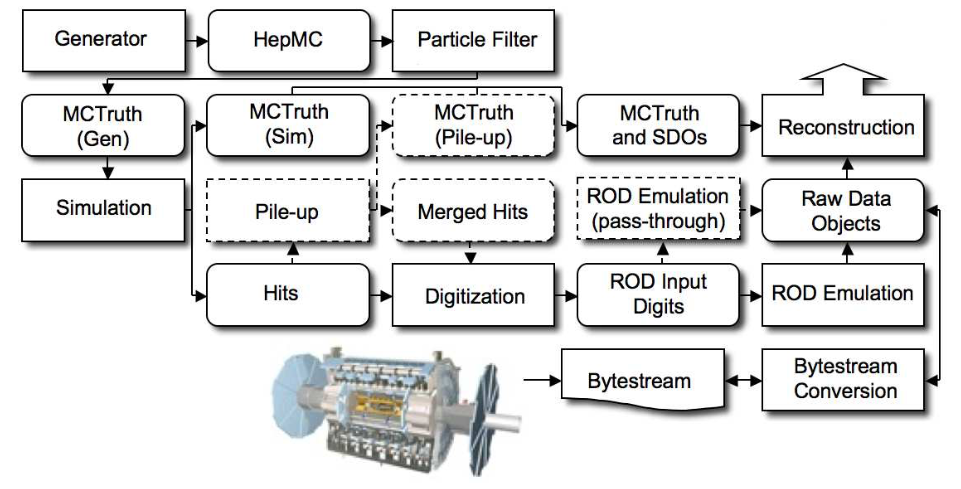
\includegraphics[scale=0.5]{images/atlas_sim_chain}
\caption{An illustration showing the ATLAS simulation chain. The boxes with the rounded corners represent persistent data objects, while those with sharp corners represent algorithms or applications. Optional algorithms have boxes made of dashed lines. \cite{ATLAS_sim}}
\label{sim_chain}
\end{figure}